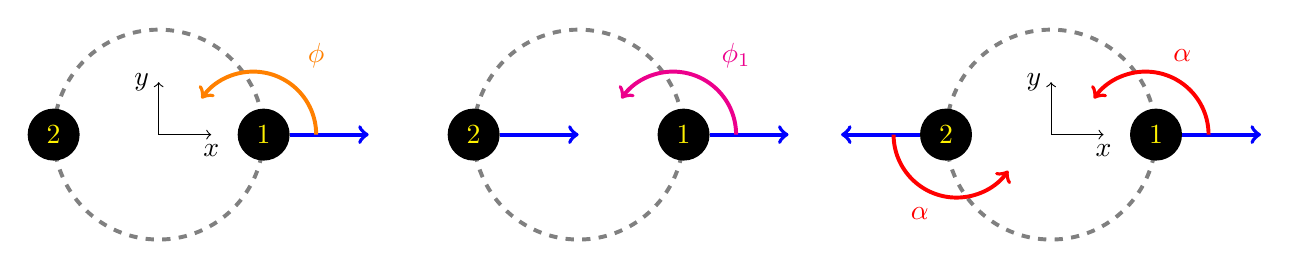
\begin{tikzpicture}

    % coordinate system
    \draw[->] (-5.333, 0) -- (-5.333, 0.666); 
    \draw[->] (-5.333, 0) -- (-4.666, 0); 
    \node[left] at (-5.333, 0.666) {$y$};
    \node[below] at (-4.666, 0) {$x$};
    \draw[->] (6, 0) -- (6, 0.666); 
    \draw[->] (6, 0) -- (6.666, 0); 
    \node[left] at (6, 0.666) {$y$};
    \node[below] at (6.666, 0) {$x$};

    % left
    \draw[dashed, gray, line width=0.5mm] (-5.333, 0) circle(1.333);
    \fill (-4, 0) circle (0.33);
    \fill (-6.667, 0) circle (0.33);
    \node[orange] at (-3.333, 1) {$\phi$};
    \node[yellow] at (-4, 0) {$1$};
    \node[yellow] at (-6.667, 0) {$2$};
    \draw[->, blue, line width=0.5mm] (-3.666, 0) -- (-2.666, 0); 
    \draw [->, orange, line width=0.5mm] (-3.333, 0) arc[start angle=0, end angle=145, radius=0.8];

    % middle 
    \draw[dashed, gray, line width=0.5mm] (0, 0) circle(1.333);
    \fill (1.333, 0) circle (0.33);
    \fill (-1.333, 0) circle (0.33);
    \node[magenta] at (2, 1) {$\phi_1$};
    \node[yellow] at (1.333, 0) {$1$};
    \node[yellow] at (-1.333, 0) {$2$};
    \draw[->, blue, line width=0.5mm] (1.666, 0) -- (2.666, 0); 
    \draw[->, blue, line width=0.5mm] (-1, 0) -- (0, 0); 
    \draw [->, magenta, line width=0.5mm] (2, 0) arc[start angle=0, end angle=145, radius=0.8];
    
    % right 
    \draw[dashed, gray, line width=0.5mm] (6, 0) circle(1.333);
    \fill (7.333, 0) circle (0.33);
    \fill (4.666, 0) circle (0.33);
    \node[red] at (7.666, 1) {$\alpha$};
    \node[red] at (4.333, -1) {$\alpha$};
    \node[yellow] at (7.333, 0) {$1$};
    \node[yellow] at (4.666, 0) {$2$};
    \draw[->, blue, line width=0.5mm] (7.666, 0) -- (8.666, 0); 
    \draw[->, blue, line width=0.5mm] (4.333, 0) -- (3.333, 0); 
    \draw [->, red, line width=0.5mm] (8, 0) arc[start angle=0, end angle=145, radius=0.8];
    \draw [->, red, line width=0.5mm] (4, 0) arc[start angle=180, end angle=325, radius=0.8];
    
\end{tikzpicture}

